\documentclass{beamer}
\usepackage[utf8]{inputenc}
\usepackage{amsmath}
\usepackage{svg}
\usepackage{biblatex}[backend=biber]
\usepackage{pgfplots}
\usepackage{listings}

\lstset{
    language=C,
    basicstyle=\ttfamily\small,
    keywordstyle=\color{blue}\bfseries,
    commentstyle=\color{green!60!black}\itshape,
    stringstyle=\color{red},
    showstringspaces=false,
    % numbers=left,
    % numberstyle=\tiny\color{gray},
    % stepnumber=1,
    % numbersep=8pt,
    tabsize=4,
    breaklines=true,
    breakatwhitespace=true,
    morekeywords={inline} % recognize 'inline'
}

\addbibresource{ref.bib}

\usetheme{Madrid}
\usecolortheme{default}

\title[ELE 548: Final Presentation]
{ELE 548: Final Presentation}

\author
{Calvin Higgins}

\institute[]
{
  Department of Computer Science and Statistics\\
  University of Rhode Island
}

\AtBeginSection[]
{
  \begin{frame}
    \frametitle{Table of Contents}
    \tableofcontents[currentsection]
  \end{frame}
}

\begin{document}

% ------------------------------------------------------------
% Slide
% ------------------------------------------------------------

\frame{\titlepage}

% ------------------------------------------------------------
% Slide
% ------------------------------------------------------------

\begin{frame}
\frametitle{Project Overview}

\begin{figure}
    \centering
    \includegraphics[scale=0.25]{approach.png}
    \caption{Reinforcement learning for the phase-ordering problem. Adapted from \cite{chaoyi2025}.}
\end{figure}

\end{frame}


% ------------------------------------------------------------
% Slide
% ------------------------------------------------------------

\begin{frame}
\frametitle{CompilerGym}

\begin{figure}
    \centering
    \includegraphics[scale=0.15]{compilergym.png}
    \caption{CompilerGym architecture~\cite{cummins2022}.}
\end{figure}

\end{frame}

% ------------------------------------------------------------
% Slide
% ------------------------------------------------------------

\begin{frame}
\frametitle{Deep Q-Network Rollout}

\begin{figure}
    \centering
    \includegraphics[scale=0.25]{rollout.png}
\end{figure}

\end{frame}

% ------------------------------------------------------------
% Slide
% ------------------------------------------------------------

\begin{frame}
\frametitle{Deep Q-Network Training}

\begin{figure}
    \centering
    \includegraphics[scale=0.25]{train.png}
\end{figure}

\end{frame}

% ------------------------------------------------------------
% Slide
% ------------------------------------------------------------

\begin{frame}
\frametitle{QSort ($n=1$)}


\begin{figure}
    \centering
    \includegraphics[scale=0.6]{qsort_improvement_factor.png}
\end{figure}

\end{frame}

% ------------------------------------------------------------
% Slide
% ------------------------------------------------------------

\begin{frame}
\frametitle{Tensorflow~\cite{abadi2016} ($n=1985$)}

\begin{center}
    \includegraphics[scale=0.6]{tensorflow_improvement_factor.png}
\end{center}

\end{frame}

% ------------------------------------------------------------
% Slide
% ------------------------------------------------------------

\begin{frame}
\frametitle{Tensorflow~\cite{abadi2016} ($n=1985$)}

\begin{center}
    \includegraphics[scale=0.4]{bug.png}
\end{center}

\begin{center}
    \Large
    \textcolor{red}{\textbf{Some programs are optimized to size zero?!}}    
\end{center}

\end{frame}

% ------------------------------------------------------------
% Slide
% ------------------------------------------------------------

\begin{frame}[fragile]
\frametitle{Example Zero Size Program}

\begin{lstlisting}
struct item_head { int dummy; };

int IH_SIZE; 
int memcpy (
    struct item_head *to, 
    const struct item_head *from, 
    int size
); 

inline void copy_item_head(
    struct item_head *to,
    const struct item_head *from
) {
    memcpy(to, from, IH_SIZE);
}
\end{lstlisting}

\begin{center}
    \Large
    \textcolor{red}{\textbf{Only inline function definitions and globals...}}    
\end{center}

\end{frame}

% ------------------------------------------------------------
% Slide
% ------------------------------------------------------------

\begin{frame}
\frametitle{ISO C Standard (n3467) Section 6.7.5.8}
\begin{quote}
Any function with internal linkage can be an inline function. For a function with external linkage,
the following restrictions apply: \textcolor{blue}{\textbf{If all the file scope declarations for a function in a translation unit
include the inline function specifier without extern, then the definition in that translation unit
is an inline definition. An inline definition does not provide an external definition for the function}}
and does not forbid an external definition in another translation unit. 
\end{quote}

\begin{center}
    \Large
    \textcolor{red}{\textbf{Inline functions are only available inside the file where they are defined!}}    
\end{center}

\end{frame}

% ------------------------------------------------------------
% Slide
% ------------------------------------------------------------

\begin{frame}
\frametitle{Hyperparameter Sweep}

\begin{center}
\begin{figure}
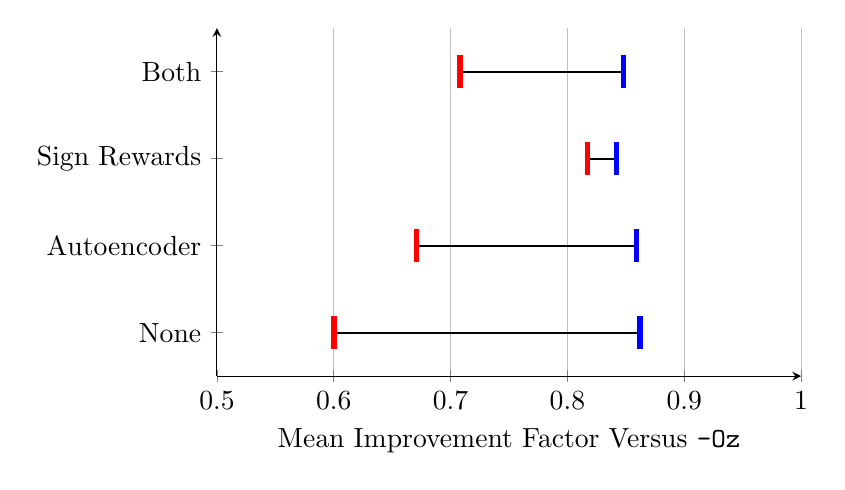
\begin{tikzpicture}
\begin{axis}[
    xmajorgrids,
    xlabel={Mean Improvement Factor Versus \texttt{-Oz}},
    ytick={1,2,3,4},
    yticklabels={None, Autoencoder, Sign Rewards, Both},
    width=9cm,
    height=6cm,
    xmin=0.5,
    xmax=1,
    ymin=0.5,
    ymax=4.5,
    enlarge y limits=0.15,
    axis y line=left,
    axis x line=bottom,
]

\addplot+[thick, black, mark=none, line cap=round] coordinates { (0.600,1) (0.862,1) } node[right,pos=0.95] {}; 
\addplot+[thick, black, mark=none, line cap=round] coordinates { (0.671,2) (0.859,2) } node[right,pos=0.95] {};
\addplot+[thick, black, mark=none, line cap=round] coordinates { (0.817,3) (0.842,3) } node[right,pos=0.95] {};
\addplot+[thick, black, mark=none, line cap=round] coordinates { (0.708,4) (0.848,4) } node[right,pos=0.95] {};

\addplot+[
    only marks,
    mark=|,
    mark size=6pt,
    mark options={line width=2pt, solid, red}
    ] coordinates { (0.600,1) (0.671,2) (0.817,3) (0.708,4) };
\addplot+[only marks, mark=|, mark size=6pt, mark options={line width=2pt, solid}, blue] coordinates { (0.862,1) (0.859,2) (0.842,3) (0.848,4) };

\end{axis}
\end{tikzpicture}
\caption{Geometric mean improvement factor versus \texttt{-Oz} across six benchmark suites. Blue (red) line is maximum (minimum) improvement factor in hyperparameter sweep. All models trained on AnghaBench~\cite{dasilva2021} with Autophase~\cite{hajali2020} features (1024 episodes, 64 steps).}
\end{figure}
\end{center}

\end{frame}

% ------------------------------------------------------------
% Slide
% ------------------------------------------------------------

\begin{frame}
\frametitle{Deep Q-Network Training with Autoencoder}

\begin{figure}
    \centering
    \includegraphics[scale=0.5]{presentation-train.png}
\end{figure}

\end{frame}

% ------------------------------------------------------------
% Slide
% ------------------------------------------------------------

\begin{frame}
\frametitle{Final Results: BLAS~\cite{blas2002} ($n=300$)}

\begin{center}
\begin{tikzpicture}
\begin{axis}[
    ybar,
    bar width=15pt,
    width=10cm,
    height=7cm,
    ylabel={Mean Improvement Factor Versus \texttt{-Oz}},
    symbolic x coords={\texttt{-O0}, Mine, Random Search, \texttt{-Oz}, CompilerDream},
    xtick=data,
    nodes near coords,
    ymin=0,
    x tick label style={rotate=45, anchor=east} 
]
\addplot coordinates {(\texttt{-O0},0.931) (Mine,0.951) (Random Search,0.96) (\texttt{-Oz},1.0) (CompilerDream,0.991)};
\end{axis}
\end{tikzpicture}
\end{center}

\end{frame}

% ------------------------------------------------------------
% Slide
% ------------------------------------------------------------

\begin{frame}
\frametitle{Final Results: cBench~\cite{fursin2014} ($n=23$)}

\begin{center}
\begin{tikzpicture}
\begin{axis}[
    ybar,
    bar width=15pt,
    width=10cm,
    height=7cm,
    ylabel={Improvement Factor Versus \texttt{-Oz}},
    symbolic x coords={\texttt{-O0}, Mine, Random Search, \texttt{-Oz}, CompilerDream},
    xtick=data,
    nodes near coords,
    ymin=0,
    x tick label style={rotate=45, anchor=east} 
]
\addplot coordinates {(\texttt{-O0},0.481) (Mine,0.883) (Random Search,0.858) (\texttt{-Oz},1.0) (CompilerDream,1.036)};
\end{axis}
\end{tikzpicture}
\end{center}

\end{frame}

% ------------------------------------------------------------
% Slide
% ------------------------------------------------------------

\begin{frame}
\frametitle{Final Results: CHStone~\cite{hara2008} ($n=12$)}

\begin{center}
\begin{tikzpicture}
\begin{axis}[
    ybar,
    bar width=15pt,
    width=10cm,
    height=7cm,
    ylabel={Improvement Factor Versus \texttt{-Oz}},
    symbolic x coords={\texttt{-O0}, Mine, Random Search, \texttt{-Oz}, CompilerDream},
    xtick=data,
    nodes near coords,
    ymin=0,
    x tick label style={rotate=45, anchor=east} 
]
\addplot coordinates {(\texttt{-O0},0.487) (Mine,0.940) (Random Search,1.037) (\texttt{-Oz},1.0) (CompilerDream,1.094)};
\end{axis}
\end{tikzpicture}
\end{center}
\end{frame}

% ------------------------------------------------------------
% Slide
% ------------------------------------------------------------

\begin{frame}
\frametitle{Final Results: MiBench~\cite{guthaus2001} ($n=40$)}

\begin{center}
\begin{tikzpicture}
\begin{axis}[
    ybar,
    bar width=15pt,
    width=10cm,
    height=7cm,
    ylabel={Improvement Factor Versus \texttt{-Oz}},
    symbolic x coords={\texttt{-O0}, Mine, Random Search, \texttt{-Oz}, CompilerDream},
    xtick=data,
    nodes near coords,
    ymin=0,
    x tick label style={rotate=45, anchor=east} 
]
\addplot coordinates {(\texttt{-O0},0.389) (Mine,0.745) (Random Search,1.005) (\texttt{-Oz},1.0) (CompilerDream,1.006)};
\end{axis}
\end{tikzpicture}
\end{center}
\end{frame}

% ------------------------------------------------------------
% Slide
% ------------------------------------------------------------

\begin{frame}
\frametitle{Final Results: NPB ($n=122$)}

\begin{center}
\begin{tikzpicture}
\begin{axis}[
    ybar,
    bar width=15pt,
    width=10cm,
    height=7cm,
    ylabel={Improvement Factor Versus \texttt{-Oz}},
    symbolic x coords={\texttt{-O0}, Mine, Random Search, \texttt{-Oz}, CompilerDream},
    xtick=data,
    nodes near coords,
    ymin=0,
    x tick label style={rotate=45, anchor=east} 
]
\addplot coordinates {(\texttt{-O0},0.530) (Mine,0.884) (Random Search,1.074) (\texttt{-Oz},1.0) (CompilerDream,1.108)};
\end{axis}
\end{tikzpicture}
\end{center}
\end{frame}

% ------------------------------------------------------------
% Slide
% ------------------------------------------------------------

\begin{frame}
\frametitle{Final Results: OpenCV~\cite{culjak2012} ($n=442$)}

\begin{center}
\begin{tikzpicture}
\begin{axis}[
    ybar,
    bar width=15pt,
    width=10cm,
    height=7cm,
    ylabel={Improvement Factor Versus \texttt{-Oz}},
    symbolic x coords={\texttt{-O0}, Mine, Random Search, \texttt{-Oz}, CompilerDream},
    xtick=data,
    nodes near coords,
    ymin=0,
    x tick label style={rotate=45, anchor=east} 
]
\addplot coordinates {(\texttt{-O0},0.981) (Mine,0.978) (Random Search,1.080) (\texttt{-Oz},1.0) (CompilerDream,1.092)};
\end{axis}
\end{tikzpicture}
\end{center}
\end{frame}

% ------------------------------------------------------------
% Slide
% ------------------------------------------------------------

\begin{frame}
\frametitle{Future Work}

\textbf{CompilerGym:}
\begin{enumerate}
    \item Fix race conditions
    \item Parallelize compilation
    \item Improve performance (inst2vec~\cite{bennun2018})
    \item Bump versions
\end{enumerate}

\vspace{1em}

\textbf{Program Representation:}
\begin{enumerate}
    \item Try Transformer-based embedding models
\end{enumerate}

\vspace{1em}

\textbf{Architecture:}
\begin{enumerate}
    \item Implement EfficientZero~\cite{ye2021}
\end{enumerate}

\vspace{1em}

\textbf{Objective:}
\begin{enumerate}
    \item Test runtime, energy and binary size
\end{enumerate}


\end{frame}

% ------------------------------------------------------------
% Slide
% ------------------------------------------------------------

\begin{frame}[allowframebreaks]
\frametitle{References}

\printbibliography

\end{frame}

\end{document}